% Paper 2 --- IEEE IEEEtran conversion
% Generated: 2026-11-16
% Source: PAPER2_FULL_MANUSCRIPT_DRAFT.md
% Status: DRAFT --- requires author/affiliation fill-in and figure file placement

\documentclass[journal]{IEEEtran}

\usepackage{amsmath}
\usepackage{graphicx}
\usepackage{booktabs}
\usepackage{hyperref}
\usepackage{url}
\usepackage{cite}

% -----------------------------------------------------------------------
\begin{document}

\title{Geographically Grouped Federated and Centralized Regression for
Conditional Harvest Prediction in Cereal-Legume Field Experiments}

\author{[Author Name(s)]\thanks{Manuscript submitted 2026-11-16.
Correspondence: [email].}}

\maketitle

% -----------------------------------------------------------------------
\begin{abstract}
Agricultural prediction across research locations is complicated by unequal
sample sizes, heterogeneous crop support, and the risk that pooled metrics hide
failures in small or held-out groups. This study evaluates centralized and
simulated horizontal federated learning for retrospective conditional harvest
seed-dry-matter regression using 607 recorded cereal-legume crop-management
systems from eight geographic groups. A nested group-held-out protocol was used
for validation and outer evaluation, with training-only preprocessing, five
declared refit seeds, immutable execution identities, and one-time test-inference
receipts. In the original eight-method comparison, XGBoost had the lowest
observed equal-group RMSE (1.2461 t/ha) and pooled RMSE (1.7335 t/ha), while the
evaluated neural models exhibited severe extrapolation from input columns that
were unsupported during training. A training-only zero-support guard reduced
these neural errors in a post-hoc fixed-model sensitivity analysis and is not
treated as independent confirmation. A later prospectively frozen fixed-public
refit achieved equal-group RMSE $1.067407 \pm 0.021053$ t/ha and pooled RMSE
$1.201189 \pm 0.038476$ t/ha. In its matched aggregation-noise study, equal-group
RMSE increased to 1.182853, 2.218085, and 5.628243 t/ha at noise multipliers 2,
4, and 8, respectively. Equal-group and pooled metrics, geographic results, and
seen/unseen support panels are reported together. The study provides a
reproducible characterization of grouped conditional regression and controlled
noise utility; it does not establish best-crop recommendation, causal
agricultural benefit, a novel federated optimizer, independent field
generalization, secure aggregation, or end-to-end differential privacy.
\end{abstract}

\begin{IEEEkeywords}
Agricultural regression, cereal-legume systems, federated learning, grouped
validation, FedAvg, FedProx, FedNova, model support, aggregation noise,
reproducibility.
\end{IEEEkeywords}

% -----------------------------------------------------------------------
\section{Introduction}

Agricultural outcome models are often developed from observations collected at
several locations, seasons, and experimental sites. These data are valuable
precisely because the environments differ, yet that variation also complicates
evaluation. A model can perform well when records from a well-represented site
dominate a pooled test set while remaining unreliable at smaller or previously
held-out locations. The distinction matters for cereal-legume experiments, in
which species composition, management, climate, and measurement support are
not evenly distributed across research groups.

Federated learning offers a way to coordinate model fitting without combining
all client records in one training table. The core algorithms are already well
established: FedAvg \cite{mcmahan2017communication} aggregates locally updated
models, FedProx \cite{li2020fedprox} adds a proximal term for heterogeneous
clients, and FedNova \cite{wang2020fednova} normalizes local updates to address
objective inconsistency. Their availability does not remove the
experimental-design problem: agricultural clients may have unequal sample sizes
and disjoint biological support, and pooled metrics may answer a different
question from metrics that weight held-out groups equally.

This study examines that problem using 607 recorded cereal-legume
crop-management systems from eight geographic groups. The target is complete
harvest seed dry matter, expressed in t/ha, for an observed system. Species
composition is an input condition rather than a recommended label. We therefore
formulate the task as retrospective conditional regression, not as best-crop
selection, causal treatment comparison, or a claim that changing a system will
improve yield.

The study asks three questions. First, how do conventional centralized and
simulated horizontal federated baselines behave when each geographic group is
held out in turn? Second, how does interpretation change between equal-group
and pooled evaluation, particularly when group sizes and species support are
unequal? Third, what utility degradation is observed when prospectively matched
clipping and Gaussian aggregation-noise variants are applied to a fixed-public
representation? The third question is deliberately restricted to a utility
simulation. It does not establish end-to-end differential privacy, secure
aggregation, or a deployable private system.

The contributions are methodological and evidential:
\begin{enumerate}
  \item a versioned nested group-held-out protocol with training-only
        preprocessing, immutable data and code identities, validation-only model
        selection, five declared refit seeds, and one-time outer-inference
        receipts;
  \item a complete comparison of training-mean, ridge, random-forest, XGBoost,
        centralized-MLP, FedAvg, FedProx, and restricted-FedNova baselines under
        the same conditional harvest-regression task;
  \item reporting that separates equal-group from pooled metrics and includes
        regional and seen/unseen species-composition support panels, rather than
        suppressing adverse or small-group results;
  \item a separately identified post-hoc support sensitivity and a prospectively
        frozen matched clipping/noise simulation whose limitations are retained
        in the evidence record; and
  \item reproducibility assets linking plans, source and data hashes, attempts,
        cached predictions, independent audits, exact plot values, and manuscript
        claims.
\end{enumerate}

These contributions characterize model behavior within one retrospective
benchmark. They do not establish a new federated optimizer, agronomic knowledge
guidance, numerical superiority to published studies, formal production
privacy, independent field generalization, or agricultural benefit.

% -----------------------------------------------------------------------
\section{Related Work}

\subsection{Federated Optimization Under Heterogeneous Clients}

FedAvg \cite{mcmahan2017communication} introduced communication-efficient
iterative averaging of models trained on decentralized data. FedProx
\cite{li2020fedprox} modified the local objective with a proximal penalty
intended to improve optimization under systems and statistical heterogeneity.
FedNova \cite{wang2020fednova} addressed objective inconsistency caused by
unequal local work through normalized updates. Paper 2 uses these methods as
established baselines. Its restricted implementations and shared evaluation
budget are documented explicitly; no convergence theorem or novelty claim is
inherited from the original papers.

Agricultural heterogeneity also has a support dimension that aggregation alone
does not solve. A held-out group may contain a species or composition absent
from all training groups, while a large group may dominate a pooled metric.
For this reason, the present study reports equal-group and pooled summaries
together and provides support-conditioned panels. These summaries are
descriptive for the benchmark and are not geographic confidence intervals.

\subsection{Federated Agricultural Yield Prediction}

Federated crop-yield prediction predates this study. A 2022 DELCON study
\cite{delcon2022yield} applied FedAvg with residual networks to soybean-yield
regression. Li et al.\ later proposed federated model pruning
\cite{li2024pruning} for localized and efficient soybean-yield forecasting.
These papers are the closest horizontal yield-regression contexts, but their
crops, records, client construction, model objectives, splits, metrics, and
computational budgets do not match the experimental-system benchmark used here.

Other studies broaden the systems and modeling choices. Mukherjee and Buyya
\cite{mukherjee2025architectures} compared centralized and decentralized
federated architectures with a crop-yield application. Dey et al.\
\cite{dey2025flyer} presented the edge/cloud recurrent FLyer framework, while
Nirosha and Vennila \cite{nirosha2025enhancing} combined graph and recurrent
components in a federated yield model. These works demonstrate that recurrent,
hybrid, edge/cloud, and decentralized agricultural federation are established
directions; they are not matched numeric baselines for the present task.

Recent studies also illustrate materially different definitions of clients.
Utku et al.\ \cite{utku2026forecasting} studied multi-country cereal-yield
forecasting with annual country clients and a time-aware split. Koksal et al.\
\cite{koksal2026vertical} examined vertical federated crop-yield prediction
across feature holders. The former is relevant to non-IID cereal forecasting,
but country-year time series differ from crop-management systems and held-out
experimental groups. The latter partitions features vertically, whereas Paper 2
simulates horizontal clients defined by training research groups.

Cowlishaw et al.\ \cite{cowlishaw2025balancing} evaluated client count,
imbalance, and aggregation for Earth-observation agricultural predictions. That
study used crop-type segmentation as a proxy because suitable yield data were
unavailable at the required resolution. It informs the discussion of
agricultural client heterogeneity, but a remote-sensing segmentation task is not
direct evidence for conditional harvest regression.

Accordingly, published scores are described only in their source-specific
contexts. We do not rank Paper 2 against external numbers because the target
definitions and units, populations, client construction, partitions, metrics,
and training budgets are not aligned.

\subsection{Grouped Evaluation and Support-Aware Reporting}

The central evaluation unit in Paper 2 is the geographic group, not an
independently sampled record. Inner model selection leaves out one training
group at a time, and outer evaluation holds out each of eight groups. This
design reduces direct site leakage but cannot create biological support that is
absent from training data. We therefore accompany aggregate error with
group-level results and seen/unseen species-composition panels. The analysis
also keeps a training-derived zero-support guard separate because it was
designed after original outer failures had been observed.

This protocol should not be interpreted as independent multi-region field
confirmation. The records come from one compiled experimental resource
\cite{gaudio2024cereallegume}, geographic support is unequal, and cultivar,
density, and other management variables are not sufficiently harmonized for
causal or recommendation claims.

\subsection{Privacy Mechanisms and Simulation Scope}

Federated optimization limits routine centralization of raw client tables, but
that property alone is not a formal privacy guarantee. Differentially private
training requires an explicit protected unit, clipping and noise mechanism,
composition accountant, release transcript, and threat model. Secure aggregation
is a separate cryptographic requirement intended to hide individual client
updates from the aggregator, as formalized in established protocols such as that
of Bonawitz et al.\ \cite{bonawitz2017secure}. The Gaussian accounting used in
the project follows the stated zCDP composition relationship
\cite{bun2016concentrated}, but the application-level conditions required for a
certified release are not closed.

Paper 2 therefore reports only a matched aggregation-noise utility simulation.
The unnoised control and noisy variants share the fixed-public representation,
selected settings, seeds, and evaluation protocol. This isolates observed
utility changes under the implemented simulation, but it does not demonstrate
production secure aggregation, private preprocessing, protection from gradient
inversion or membership inference, or end-to-end differential privacy.

\subsection{Position Relative to Prior Work}

The literature supports neither a first federated-yield claim nor a numerical
superiority claim. The narrower value of Paper 2 is its auditable evaluation of
conditional harvest regression across grouped experimental support: complete
baseline and adverse-result reporting, explicit equal-group versus pooled
interpretation, support panels, separation of prospective and post-hoc stages,
and a matched noise-utility study. Whether these findings transfer to new sites,
farm decisions, or established private deployments remains an open question.

% -----------------------------------------------------------------------
\section{Data and Problem Formulation}

\subsection{Source Data and Unit of Analysis}

The active benchmark was constructed from version 2.0.0 of a compiled dataset
of cereal-legume field experiments \cite{gaudio2024cereallegume}. The source
contained 37 experiments at nine site labels and covered eight crop species. We
treated neither individual trait records nor crop components within an intercrop
as independent observations. Instead, one analysis row represented one
\texttt{(experiment\_id, management)} crop system. A row was retained only when
every expected crop component had a verified complete-harvest seed dry-matter
outcome. Component outcomes were summed for intercrops, producing 607
crop-management systems.

The response for system $i$ was harvested seed dry matter,
\[
  y_i = \sum_{c \in \mathcal{C}_i} y_{ic},
\]
where $\mathcal{C}_i$ is the set of crop components in the recorded system and
the response unit is t/ha. The prediction problem was
\[
  \hat{y}_i = f(\mathbf{x}_i, \mathbf{s}_i, \mathbf{m}_i),
\]
where $\mathbf{x}_i$ denotes recorded soil and contextual variables,
$\mathbf{s}_i$ identifies the observed species composition, and $\mathbf{m}_i$
contains recorded management quantities. Crop composition was therefore an input
condition, not a recommended class. The estimand was the conditional outcome of
a recorded treatment bundle. It was not a causal effect, a counterfactual yield
for untested crops, or an estimate of profitability.

\subsection{Geographic Grouping and Support}

Geographic groups were defined before model evaluation. Site labels within
1 km were merged by transitive union using source coordinates. Copenhagen and
Taastrup were approximately 0.37 km apart and were consequently treated as one
group. The resulting eight groups were Angers (75 systems), Auzeville (354),
Copenhagen+Taastrup (52), Grignon (64), Jyndevad (48), Kassel (4), Reading (4),
and Sanmarcoargentano (6). This policy prevented the two nearby Danish labels
from appearing on opposite sides of a split, but it did not establish that
broader spatial dependence was absent.

Group sizes were highly unequal: Auzeville contributed 354 of 607 systems,
whereas Kassel and Reading contributed four systems each. Biological support was
also uneven. Holding out Auzeville removed chickpea, lentil, and durum wheat
from training. We therefore recorded, for every test system, whether all of its
component species and whether its exact species composition had occurred in the
corresponding outer-training data. These indicators were derived from training
identities only and were not model inputs or outcome-dependent filters.

\subsection{Predictor Contract}

The fold-fitted baseline used seven recorded numerical quantities: soil
available water, clay fraction, soil pH, initial mineral nitrogen, applied
nitrogen, recorded phosphorus amount, and irrigation amount. Sowing date was
represented by sine and cosine calendar terms. Previous crop, crop season, and
recorded pest-control status were categorical. Eight fixed species-membership
indicators and a sole/intercrop indicator described crop composition.

Numeric medians, means, and standard deviations were estimated from each
training fold only. Missing numeric values received the training median and a
separate missingness indicator. An all-training-missing variable used a zero
computational placeholder with an explicit state flag; zero was not interpreted
as an observed measurement. Categorical vocabularies were likewise fitted on
training rows and contained distinct missing and unknown states. Depending on
the categories present in training, the encoded baseline dimension ranged from
45 to 49 across folds. Targets were neither imputed nor standardized with
held-out information.

Sand and silt were excluded because their source metadata descriptions appeared
interchanged and no correction could be independently justified. Realized
climate, actual harvest date, measured plant traits, target-derived variables,
geographic coordinates, country, year, experiment identifiers, and management
identifiers were not predictors. Cultivar and density were also excluded because
their coverage and cross-experiment comparability were unresolved. Recorded
fertilizer and irrigation values make this a retrospective conditional model;
the feature set is not certified as information available before sowing.

For the later fixed-public study, the same 607 outcomes, row identities, groups,
and partitions were re-encoded with a 54-dimensional, data-independent schema.
This transform used fixed definitions rather than training-fitted numerical
statistics or categorical vocabularies. It was introduced to make the matched
clipping/noise simulation mechanically interpretable; it did not make the
underlying records public or establish private preprocessing.

\subsection{Scientific Scope}

The dataset was used only for retrospective conditional harvest regression.
Ranking was disabled because management-matched alternatives were not verified
as randomized or comparable counterfactual choices, and cultivar, density, and
other treatment differences could not be safely collapsed. Agronomic guidance
was also disabled because no independently sourced rule passed the required
feature-unit, scope, and target-compatibility gates. Consequently, the study
does not provide best-crop labels, a validated agronomic knowledge mechanism,
or evidence of yield improvement caused by following model output.

% -----------------------------------------------------------------------
\section{Methods}

\subsection{Nested Geographic Evaluation}

We used nested leave-one-geographic-group-out evaluation. Each of the eight
groups served once as the outer test group. Within each outer-training set, each
of the remaining seven groups served once as an inner validation group, yielding
56 inner folds and eight outer refits. All rows sharing an experiment, site, or
geographic group remained on the same side of a split. Inner-fold assets
contained training and validation arrays only; outer-test arrays were omitted.

Hyperparameters were selected solely from the inner folds. Five fixed seeds
(123, 2024, 3407, 9999, and 2718) were then used for outer refitting. They
measured variability from initialization and training order; they were not five
independent agricultural replications. Final neural checkpoints were taken at a
fixed refit round derived from inner validation, with no outer-test early
stopping or checkpoint selection. Each planned run permitted one committed outer
inference. An inference intent, prediction cache, receipt, model identity,
source identity, data identity, and attempt journal were bound together; an
ambiguous interrupted inference was rejected rather than silently repeated.

\subsection{Regression Baselines}

Eight methods were evaluated. The training-mean predictor provided a constant
control. Ridge regression used candidate penalties
$\alpha \in \{0.1, 1, 10\}$. Random forest candidates used 100 trees with
minimum leaf size 1 or 3. XGBoost candidates used 100 boosting rounds, learning
rate 0.05, and maximum depth 2 or 3. Conventional candidates were selected by
equal-inner-group mean validation RMSE with first-candidate tie breaking in a
frozen order.

The shared neural regressor was
\[
  f_{\theta}(\mathbf{x}) = \mathbf{w}_2^{\mathsf{T}}
  \operatorname{ReLU}(\mathbf{W}_1 \mathbf{x} + \mathbf{b}_1) + b_2,
\]
with one hidden layer of 32 units and a scalar output. Centralized MLP, FedAvg,
FedProx, and restricted FedNova used the same architecture, initialization
scheme, mini-batch size 32, identity target scale, and mean-squared-error loss.
Optimization used constant-learning-rate SGD without momentum or weight decay.
Federated rounds used full participation and one local epoch per training group.
Logical clients were research groups in the outer-training set, not farms or
networked institutions.

For FedAvg and FedProx, selected client states were aggregated with weights
$p_k = n_k / \sum_j n_j$, where $n_k$ was the verified number of training rows
at client $k$. FedProx added the local penalty
\[
  \frac{\mu}{2}\lVert\theta - \theta_t\rVert_2^2, \qquad \mu = 0.01,
\]
relative to the round-start global model $\theta_t$. In the restricted
plain-SGD FedNova implementation, client $k$ executed $\tau_k$ mini-batch steps
and returned $\theta_k$. The server computed
\[
  \bar{\tau} = \sum_k p_k \tau_k, \qquad
  \theta_{t+1} = \theta_t - \bar{\tau} \sum_k p_k
  \frac{\theta_t - \theta_k}{\tau_k}.
\]
This formulation assumed constant local learning rate, no momentum, no weight
decay, and no proximal term. Update validation rejected missing, duplicate,
stale, non-finite, shape-incompatible, or misbound client states and checked
declared sample and step counts. These integrity checks were software safeguards,
not cryptographic client authentication.

\subsection{Inner Selection and Outer Refitting}

The original baseline search evaluated learning rates
$\{3\times10^{-4}, 10^{-3}, 3\times10^{-3}\}$ for each of the four neural
methods for 80 rounds on all 56 inner folds. A common learning rate per outer
fold was chosen by averaging validation RMSE equally across the seven inner
groups and four neural algorithms. For each algorithm, the outer-refit duration
was the median of the seven first-occurring minimum-RMSE checkpoint rounds at
the selected learning rate. This produced 1,120 completed validation candidates
and 320 outer evaluations: eight groups, five seeds, and eight methods.

The fixed search was intentionally not extended after outer outcomes were
available. Of 672 neural candidates, 286 selected the final allowed round, and
four of eight outer folds selected the highest learning rate in the grid. These
facts were retained as budget and grid-edge limitations rather than interpreted
as convergence or optimality.

\subsection{Fixed-Public Refit and Matched Noise Simulation}

A later development stage used the 54-dimensional fixed-public representation.
Its separate inner search evaluated the prospectively bounded public-transform
controls for 240 rounds. All eight outer groups selected target scale 1 and
learning rate 0.01; the median selected refit durations ranged from 106 to 149
rounds. 80 of 224 candidates reached the 240-round boundary, and 11 of 56
selected checkpoints had a worse training fit than their matched constant. These
adverse diagnostics were not removed and the grid was not enlarged after
outer-score exposure.

The unnoised fixed-public refit used equal client-slot averaging, full
participation, the same 32-unit regressor and five seeds. The matched follow-up
reused its selected learning rate, refit duration, initialization convention,
batch size, and four local SGD steps. Local gradients were clipped to L2 norm 1.
With learning rate $\eta = 0.01$, the resulting public model-update bound was
set to $C = 4\eta = 0.04$. The server averaged seven fixed client slots. For the
noisy variants it added coordinate-wise Gaussian noise calibrated to the
replacement sensitivity
\[
  \Delta = \frac{2C}{m}, \qquad m = 7,
\]
at noise multipliers 2, 4, and 8. A clipped, unnoised control isolated clipping
from noise. Noise streams were separated from data-order streams, and round
events committed atomically with checkpoints to prevent duplicate accounting
after recovery.

For a Gaussian event with coordinate standard deviation $s$, the recorded zCDP
quantity was
\[
  \rho = \frac{\Delta^2}{2s^2},
\]
summed over adaptive releases and converted at $\delta = 10^{-5}$ using
\[
  \varepsilon = \rho + 2\sqrt{\rho \log(1/\delta)}.
\]
No client-sampling amplification was assumed. This accounting described an
idealized noisy-only transcript. Nonprivate model selection, unnoised controls,
evaluation releases, deterministic research RNG, private preprocessing, and a
deployed secure-aggregation protocol were outside the guarantee. Accordingly,
the experiment was reported as a matched aggregation-noise utility simulation,
not as certified application differential privacy.

\subsection{Evaluation Measures}

For outer group $g$ containing $n_g$ systems, we computed
\[
  \operatorname{RMSE}_g = \sqrt{\frac{1}{n_g} \sum_{i \in g}(y_i - \hat{y}_i)^2}.
\]
The primary score for a seed was the arithmetic mean of the eight group RMSEs,
giving each geography equal weight. The secondary pooled RMSE was calculated
over all 607 outer predictions and therefore weighted groups by their system
counts. Equal-group and pooled MAE were reported analogously. R$^2$ was retained
as a secondary descriptive measure and recorded as unavailable for groups in
which it was undefined; it was never replaced with zero. Negative predictions
were retained rather than clipped.

Metrics were also calculated for all systems, training-seen species, training-
unseen species, training-seen exact compositions, and training-unseen exact
compositions. The all-system result remained primary, so support panels could
not hide difficult cases. Reported variability was the sample standard deviation
across the five fixed seeds. Because folds shared training data and seeds did
not create new locations, these deviations were descriptive and were not treated
as geographic confidence intervals or confirmatory significance tests.

\subsection{Reproducibility Safeguards}

Plans were frozen before their corresponding outer inference stages. Execution
was bounded and resumable under an exclusive writer lock. Manifests bound raw
and prepared data, source snapshots, configurations, dependency versions, fold
identities, model assets, cached predictions, and receipts. Completed caches
were independently audited without loading models for repeat test inference.
Failures and recovery attempts were retained in journals, and existing result
directories were not overwritten. These safeguards establish local software and
evidence consistency; they do not constitute Linux deployment validation, field
validation, secure aggregation, or formal privacy certification.

% -----------------------------------------------------------------------
\section{Results}

All reported results were obtained from completed cached evaluations that passed
independent provenance and metric audits. Unless stated otherwise, values are
means $\pm$ sample standard deviation across the five fixed seeds. Standard
deviations describe computational variability; they are not confidence intervals
over independent geographic trials.

\subsection{Original Eight-Method Outer Evaluation}

The original prospectively frozen study completed 320 evaluations: eight
held-out geographic groups, five seeds, and eight methods. Table~\ref{tab:orig}
summarizes the all-system errors. Equal-group RMSE was the primary measure,
while pooled RMSE weighted each of the 607 systems equally.

\begin{table}[htbp]
\caption{Original Grouped Outer-Evaluation Results (RMSE, t/ha).}
\label{tab:orig}
\centering
\begin{tabular}{lrr}
\toprule
Method & Equal-group RMSE & Pooled RMSE \\
\midrule
XGBoost             & $1.2461 \pm 0.0000$ & $1.7335 \pm 0.0000$ \\
Random forest       & $1.3181 \pm 0.0091$ & $1.9958 \pm 0.0360$ \\
Training mean       & $1.4509 \pm 0.0000$ & $1.9379 \pm 0.0000$ \\
Ridge               & $1.4694 \pm 0.0000$ & $2.1511 \pm 0.0000$ \\
FedNova             & $5.8134 \pm 1.5956$ & $29.2405 \pm 9.8813$ \\
FedProx             & $5.8373 \pm 1.6226$ & $28.2904 \pm 9.8478$ \\
FedAvg              & $5.8373 \pm 1.6226$ & $28.2909 \pm 9.8478$ \\
Centralized MLP     & $6.0307 \pm 1.6250$ & $30.4896 \pm 10.0605$ \\
\bottomrule
\end{tabular}
\end{table}

XGBoost had the lowest observed equal-group and pooled RMSE within this frozen
benchmark. This was a descriptive result, not an inferential superiority claim.
All eight methods had negative mean pooled R$^2$; XGBoost's value was
$-0.1807$. Thus, its lower RMSE did not establish strong explained variance
across the combined held-out systems.

The gap between equal-group and pooled errors was especially large for the four
neural methods. Auzeville contained 354 of 607 systems and therefore dominated
the pooled summary. In one documented example, FedAvg at seed 123 had an
Auzeville RMSE of 36.7482 t/ha, compared with group RMSEs between approximately
0.54 and 1.76 t/ha elsewhere. The failure was retained in the original result;
neural hyperparameters and budgets were not changed after observing it.

The geographic XGBoost errors also varied despite its deterministic zero seed
SD: RMSE ranged from 0.5452 t/ha at Reading to 1.8594 t/ha at Auzeville.
Reading and Kassel contained only four systems each, so their apparently low
errors should not be interpreted as stable regional estimates.

\begin{figure}[htbp]
\centering
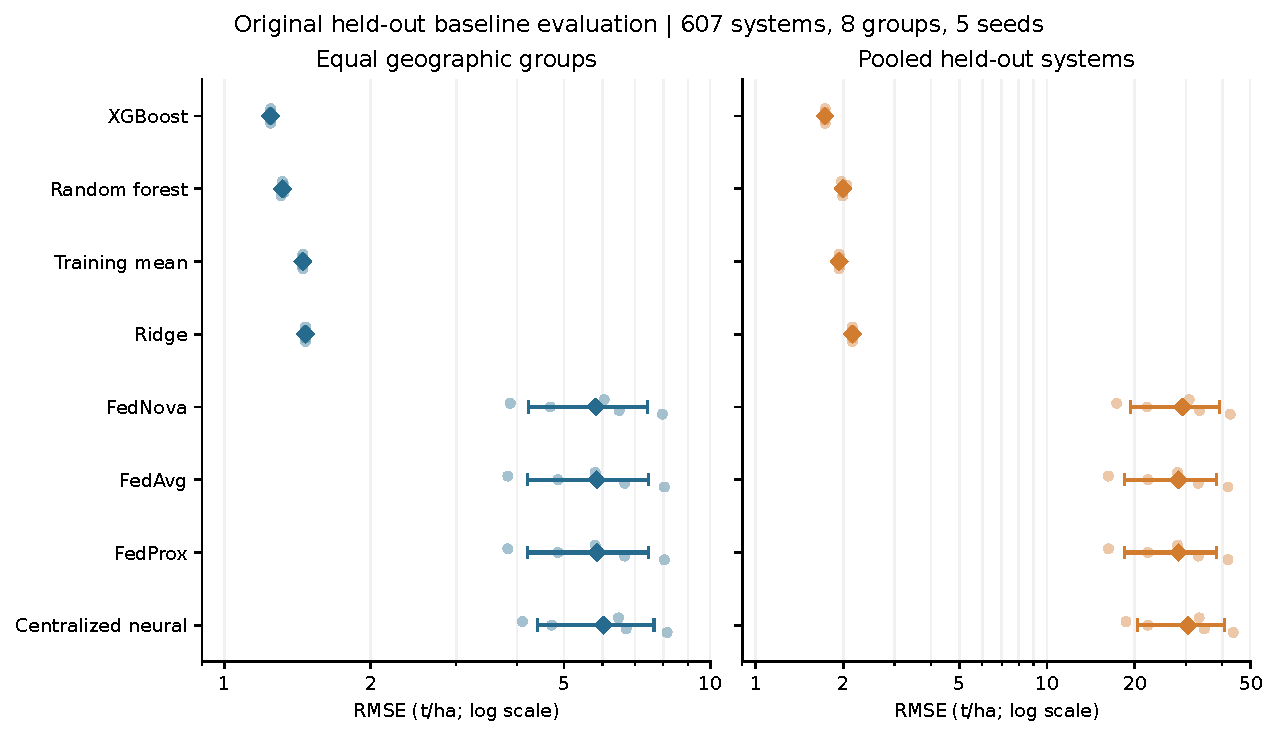
\includegraphics[width=\columnwidth]{fig_original_baseline_rmse}
\caption{Original eight-method equal-group and pooled RMSE comparison across
all methods and seeds. All seed values and group counts are shown.}
\label{fig:1}
\end{figure}

\begin{figure}[htbp]
\centering
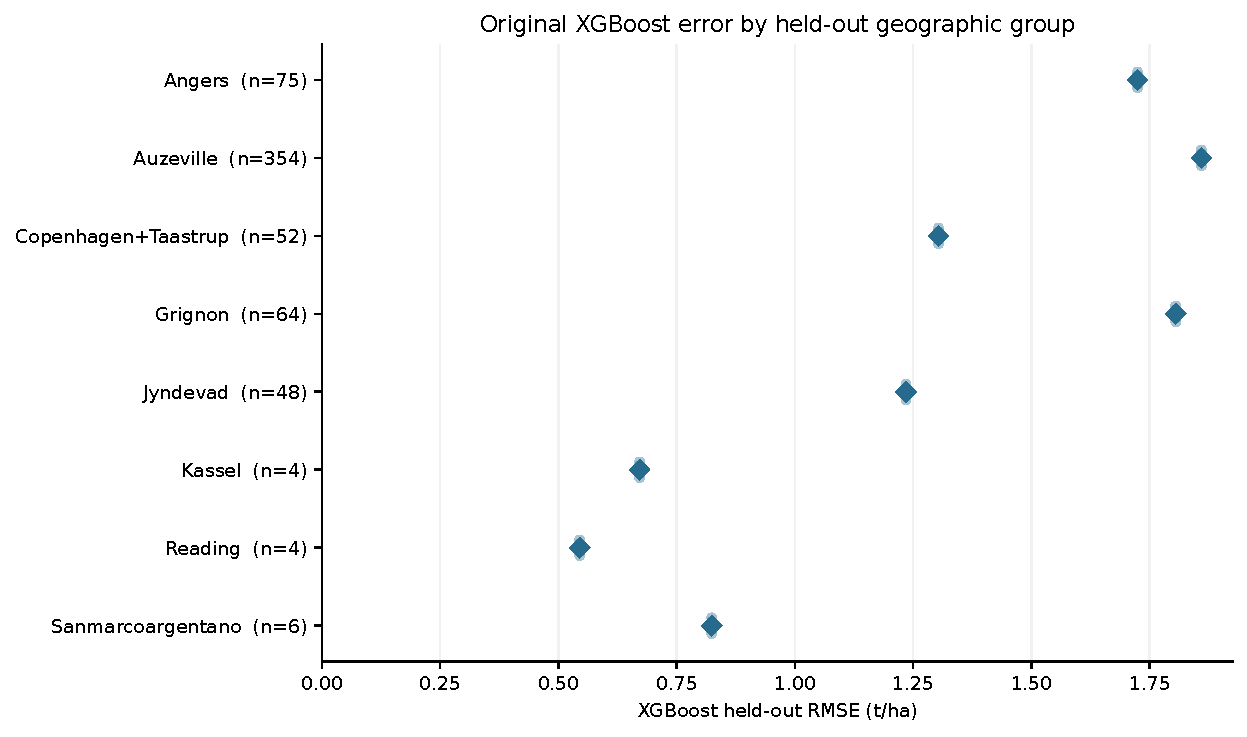
\includegraphics[width=\columnwidth]{fig_original_xgboost_geographic_rmse}
\caption{Geographic XGBoost outer RMSE across the eight held-out groups.
Group system counts are indicated.}
\label{fig:2}
\end{figure}

\subsection{Support-Conditioned and Post-Hoc Sensitivity Analysis}

Across the original splits, 342 systems had species and exact compositions seen
in the corresponding training sets. The remaining 265 systems had unseen
species/compositions, and all 265 belonged to Auzeville. Consequently, the
unseen panel represented one region rather than general cross-region
extrapolation.

Inspection after the outer failures showed that some encoded columns were zero
for every training row but nonzero in held-out data. For example, standardized
soil available water and phosphorus columns in the Auzeville holdout reached
values of approximately 263 and 66 even though both columns were identically
zero during training. A training-only zero-support guard was therefore evaluated
as a separate fixed-model sensitivity analysis. It set only all-training-zero
input columns to zero at inference and did not retrain models, change budgets,
or use outcomes to choose columns.

\begin{table}[htbp]
\caption{Post-Hoc Zero-Support Sensitivity (Equal-Group RMSE, t/ha).}
\label{tab:posthoc}
\centering
\begin{tabular}{lrr}
\toprule
Neural method & Original & Guarded post-hoc sensitivity \\
\midrule
Centralized MLP & $6.0307 \pm 1.6250$ & $1.2130 \pm 0.0196$ \\
FedAvg          & $5.8373 \pm 1.6226$ & $1.3438 \pm 0.0295$ \\
FedProx         & $5.8373 \pm 1.6226$ & $1.3438 \pm 0.0295$ \\
FedNova         & $5.8134 \pm 1.5956$ & $1.1820 \pm 0.0204$ \\
\bottomrule
\end{tabular}
\end{table}

For FedAvg at seed 123, Auzeville RMSE changed from 36.7482 to 0.9960 t/ha.
This quantifies the behavior of the specified guard but does not isolate the
effect of an individual feature or establish performance on independently
collected data. The guard was designed after outer-test failures were exposed;
therefore Table~\ref{tab:posthoc} is explicitly post-hoc and does not replace
the original prospective results.

\subsection{Fixed-Public Unnoised Refit}

The separately frozen fixed-public stage used the 54-dimensional transform and
its own inner selection. All 40 outer refits completed and passed a
cached-output audit. The primary equal-group RMSE was
$1.067407 \pm 0.021053$ t/ha; pooled RMSE was $1.201189 \pm 0.038476$ t/ha.
Equal-group MAE was $0.881704 \pm 0.022902$, pooled MAE was
$0.948698 \pm 0.043564$, and pooled R$^2$ was $0.432669 \pm 0.036004$.

Results differed across geographic groups, as shown in
Table~\ref{tab:geographic}.

\begin{table}[htbp]
\caption{Fixed-Public Unnoised Geographic Results.}
\label{tab:geographic}
\centering
\begin{tabular}{lrrr}
\toprule
Held-out group & Systems & RMSE mean $\pm$ seed SD & Mean R$^2$ \\
\midrule
Angers               & 75  & $1.657205 \pm 0.044743$ &  $0.083167$ \\
Auzeville            & 354 & $0.989938 \pm 0.059142$ &  $0.346560$ \\
Copenhagen+Taastrup  & 52  & $1.170048 \pm 0.032327$ & $-0.077797$ \\
Grignon              & 64  & $1.707368 \pm 0.061959$ & $-0.360441$ \\
Jyndevad             & 48  & $1.092247 \pm 0.053302$ &  $0.254387$ \\
Kassel               & 4   & $0.562621 \pm 0.011994$ & $-0.313808$ \\
Reading              & 4   & $0.433949 \pm 0.005893$ &  $0.662469$ \\
Sanmarcoargentano    & 6   & $0.925882 \pm 0.022788$ & $-0.109800$ \\
\bottomrule
\end{tabular}
\end{table}

\begin{figure}[htbp]
\centering
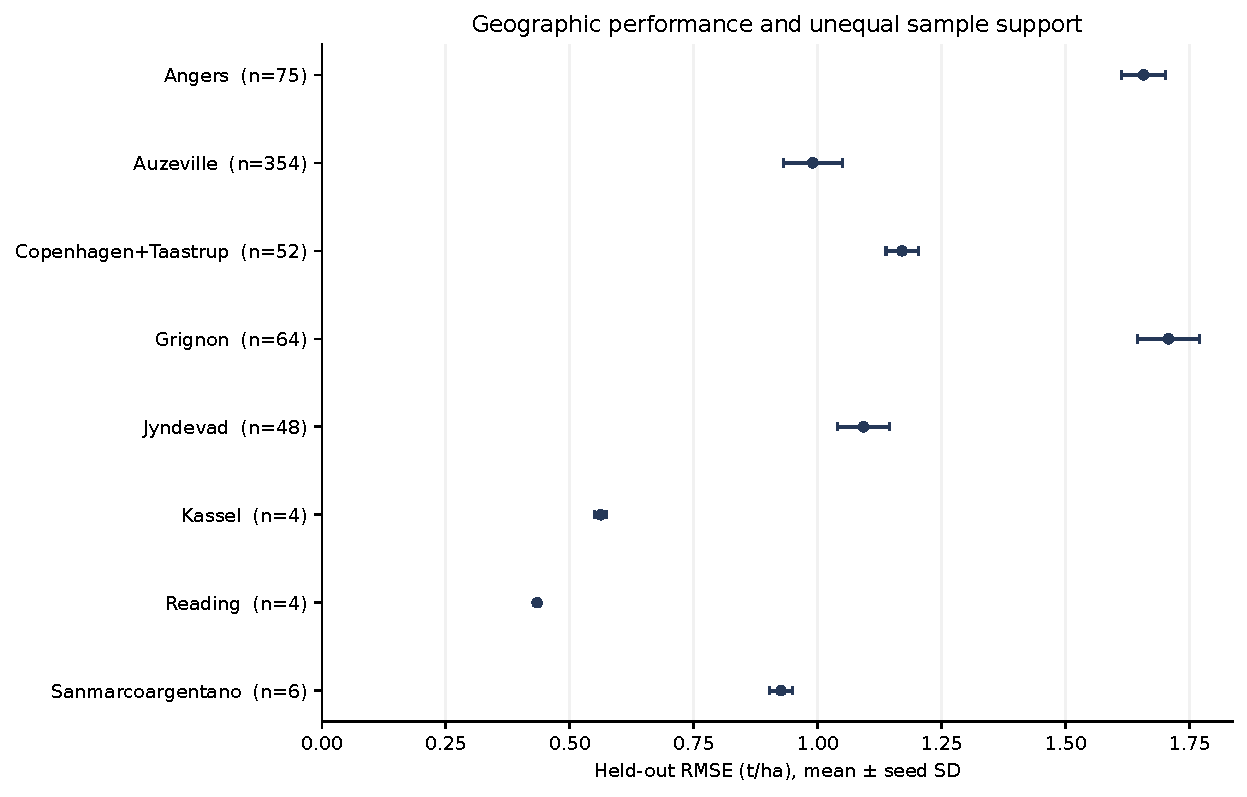
\includegraphics[width=\columnwidth]{fig_geographic_rmse}
\caption{Fixed-public geographic RMSE across the eight held-out groups, showing
seed variability and system counts.}
\label{fig:3}
\end{figure}

Four groups had negative mean R$^2$ even though overall pooled R$^2$ was
positive. The result demonstrates why pooled and equal-group summaries were
retained together and why small-group RMSE alone was insufficient for
interpretation. All 40 final training fits outperformed their matched
equal-client constant, but this did not guarantee generalization to every outer
group.

The training-seen species panel contained 342 systems from all eight groups and
had equal-group RMSE $1.070628 \pm 0.024447$ t/ha. The unseen panel contained
265 Auzeville systems and had RMSE $0.979646 \pm 0.065301$ t/ha. The lower
unseen-panel error must not be interpreted as universal unseen-species capability
because the seen and unseen panels represented different systems and geographic
distributions. Exact-composition panels had the same membership in these splits.

The fixed-public result is a later development stage with a different feature
transform, weighting rule, selection search, and refit budget from the original
eight-method study. Its numerical values are therefore not presented as a
matched correction or superiority comparison against Table~\ref{tab:orig}.

\subsection{Matched Clipping and Aggregation-Noise Utility}

The matched follow-up added 160 new evaluations and reused 40 bound unnoised
reference caches, giving eight groups and five seeds for each of five variants.
All 40 clipped-control prediction arrays exactly matched the corresponding
unnoised reference arrays. This showed no detected prediction difference in
those pairs, but per-round diagnostics were insufficient to claim that clipping
was never active.

\begin{table}[htbp]
\caption{Matched Aggregation-Noise Utility Results (RMSE, t/ha).}
\label{tab:noise}
\centering
\begin{tabular}{lrrrr}
\toprule
Variant & Equal-group RMSE & Pooled RMSE & Mean pooled R$^2$ &
  Fits worse than matched constant \\
\midrule
Cached unnoised reference & $1.067407 \pm 0.021053$ & $1.201189 \pm 0.038476$ &  $0.432669$ & $0/40$ \\
Clipped control           & $1.067407 \pm 0.021053$ & $1.201189 \pm 0.038476$ &  $0.432669$ & $0/40$ \\
Noise multiplier 2        & $1.182853 \pm 0.115717$ & $1.368078 \pm 0.120487$ &  $0.260112$ & $0/40$ \\
Noise multiplier 4        & $2.218085 \pm 0.491871$ & $2.770127 \pm 0.852787$ & $-2.243366$ & $29/40$ \\
Noise multiplier 8        & $5.628243 \pm 0.500009$ & $7.238383 \pm 1.108712$ & $-19.970877$ & $40/40$ \\
\bottomrule
\end{tabular}
\end{table}

\begin{figure}[htbp]
\centering
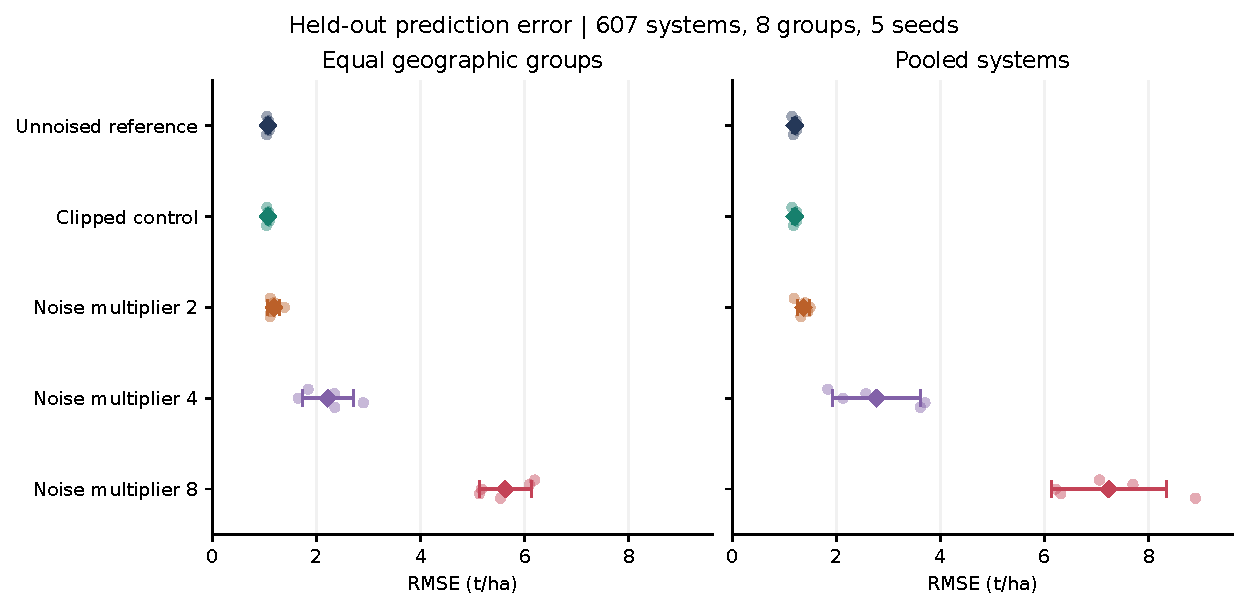
\includegraphics[width=\columnwidth]{fig_rmse_overview}
\caption{Matched aggregation-noise utility overview: equal-group and pooled RMSE
across all five variants (unnoised reference, clipped control, noise
multipliers 2, 4, and 8), with all seed values and group counts.}
\label{fig:4}
\end{figure}

\begin{figure}[htbp]
\centering
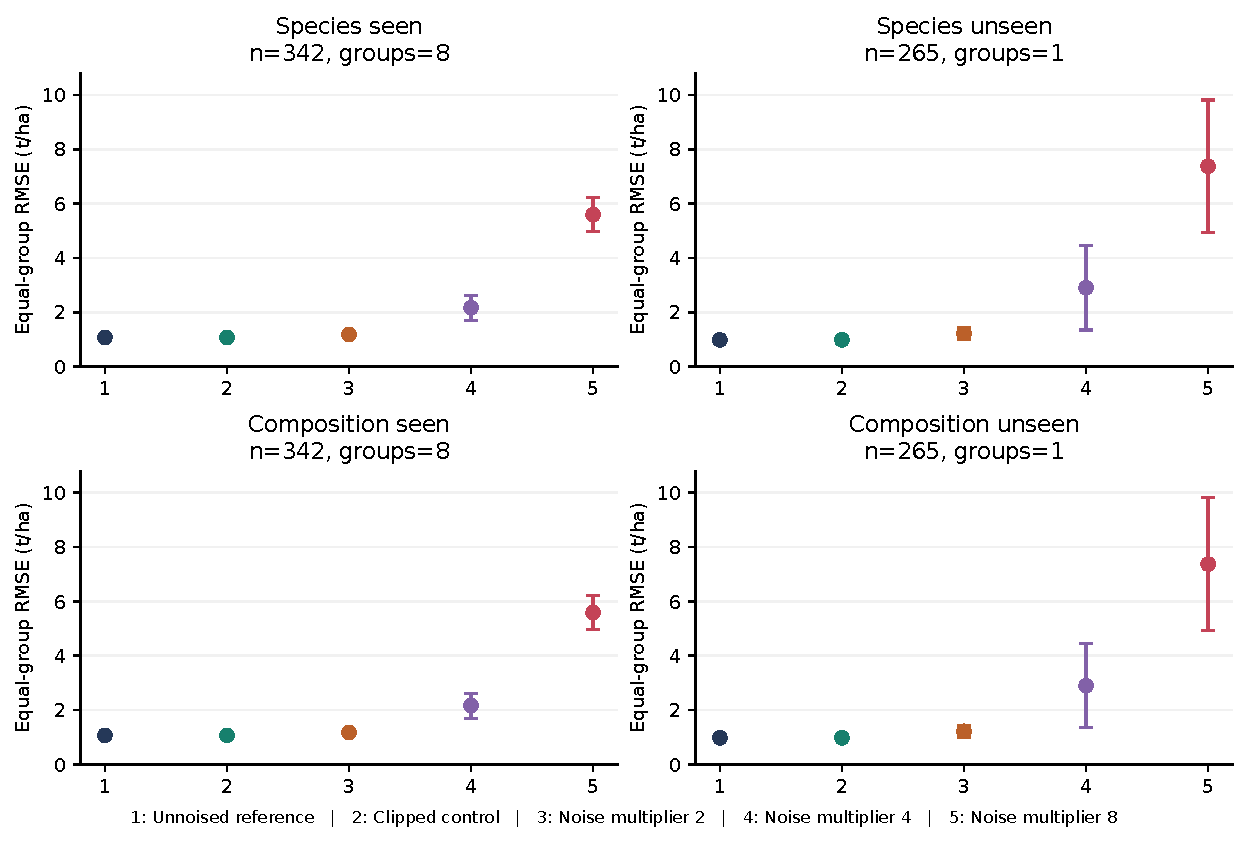
\includegraphics[width=\columnwidth]{fig_support_rmse}
\caption{Support-conditioned RMSE across noise variants, showing seen and unseen
species/composition panels with group counts.}
\label{fig:5}
\end{figure}

Mean paired increases in equal-group RMSE relative to the cached reference were
0.000000, 0.115446, 1.150678, and 4.560836 t/ha for the clipped,
multiplier-2, multiplier-4, and multiplier-8 variants, respectively. Error
increased with the noise multiplier in this fixed experiment. The large negative
R$^2$ and weak training fits at multipliers 4 and 8 were retained as adverse
findings rather than treated as execution failures.

Support-conditioned behavior also degraded with noise. At multiplier 2,
equal-group RMSE was $1.178797 \pm 0.113484$ t/ha for 342 seen systems and
$1.220762 \pm 0.216734$ t/ha for the 265 Auzeville-only unseen systems. At
multiplier 8, the corresponding values were $5.591927 \pm 0.626727$ and
$7.376316 \pm 2.435713$ t/ha.

The complete ledger contained 23,174 events: 8,564 retained historical events
and 14,610 new noisy-round events. Conditional noisy-only cumulative epsilon
bounds at $\delta = 10^{-5}$ ranged from 1297.067440 to 1377.757121 across
client slots. These values were too large to support a strong privacy claim and
did not cover nonprivate selection, controls, evaluation releases, deterministic
research randomness, or secure aggregation. The results therefore characterize
utility under controlled aggregation noise only; they do not establish
application differential privacy or production privacy.

\subsection{Summary of Empirical Findings}

Three patterns were consistent with the evidence. First, the original frozen
baseline comparison favored tree ensembles in observed RMSE, while the neural
methods exhibited severe held-out support failures. Second, a training-only
support guard greatly changed those fixed-model neural predictions, but its
post-hoc design prevents it from serving as independent confirmation. Third,
the later fixed-public matched study produced substantially better unnoised
neural errors, while stronger aggregation noise caused progressively poorer
utility and weak training fits in the evaluated setting.

These stages answer different development questions and should not be collapsed
into a single model ranking. None establishes best-crop recommendation,
agronomic benefit, universal geographic generalization, a novel federated
optimizer, or an end-to-end privacy guarantee.

% -----------------------------------------------------------------------
\section{Discussion}

\subsection{Interpreting the Baseline and Support Results}

The original grouped evaluation did not show a general advantage for neural or
federated models. XGBoost had the lowest observed equal-group and pooled RMSE,
while centralized MLP, FedAvg, FedProx, and FedNova produced severe Auzeville
errors. That outcome is scientifically useful because it shows how a seemingly
ordinary tabular preprocessing decision can interact with geographic support.
Columns that were identically zero in training could activate large,
initialization-dependent neural weights when nonzero values appeared in the
held-out group. Tree ensembles did not exhibit the same numerical failure in
this experiment, although their negative pooled R$^2$ also cautions against a
strong generalization claim.

The training-only support guard greatly reduced fixed-model neural errors, but
its interpretation is constrained by its history. It was designed after the
outer failures were visible, and the same test folds were evaluated again.
Therefore, the guarded values identify a plausible failure mechanism and a
candidate input policy; they do not erase the original result or provide
independent confirmation. A future study should specify the handling of
all-training-constant and unseen inputs before any outer evaluation and then
test that policy on new experimental groups.

The fixed-public refit further showed that stable neural behavior was possible
under a different, prospectively frozen representation and training protocol.
However, its lower RMSE cannot be attributed to federation, the fixed transform,
equal client weighting, longer refit budgets, or any one design choice in
isolation. These factors changed together, and the stage followed earlier outer
exposure. It should therefore be interpreted as a separately documented
development study rather than a matched correction to the original baseline.

\subsection{Equal-Group, Pooled, and Support-Conditioned Views}

Equal-group and pooled metrics answered different questions. Equal-group RMSE
assigned the same influence to each of eight held-out geographies, including
groups containing only four or six systems. Pooled RMSE emphasized Auzeville,
which contained 354 of 607 systems. Neither weighting was universally
preferable: the first made small-group instability influential, whereas the
second could hide poor performance outside the dominant group. Reporting both
prevented an implicit choice of estimand from being mistaken for model
improvement.

The support panels also require careful reading. All 265 systems containing
unseen species or exact compositions came from Auzeville. Their error therefore
combined biological support status with one location's target distribution and
management conditions. The apparently favorable unseen-panel result in the
fixed-public stage is not evidence that unseen crops can generally be predicted.
It instead demonstrates why support status, geography, and sample count must be
shown together.

Four fixed-public held-out groups had negative mean R$^2$ even though the pooled
R$^2$ was positive. Kassel and Reading each contained only four systems, so
their R$^2$ and RMSE were particularly sensitive to a small number of outcomes.
These adverse group-level results limit claims based only on aggregate metrics
and reinforce that five training seeds are not five independent regional trials.

\subsection{Aggregation Noise and Privacy Interpretation}

The matched study isolated utility changes under the implemented clipping and
Gaussian aggregation-noise variants. The clipped control reproduced all 40
unnoised prediction arrays exactly, while error increased at noise multipliers
2, 4, and 8. At the two larger multipliers, many or all saved fits were worse
than their matched training constant and pooled R$^2$ became strongly negative.
These outcomes were retained rather than retuned away and show the practical
cost of the evaluated noise levels under the fixed optimizer work.

This experiment does not establish an application privacy guarantee. The
conditional noisy-only composition bounds were very large, and the accounting
excluded nonprivate hyperparameter selection, unnoised controls, diagnostics,
test-metric releases, deterministic research noise seeds, and secure aggregation.
The server-side simulation also assumed a trusted curator able to inspect client
updates. Formal protection against an untrusted server would require a vetted
secure-aggregation or distributed-noise protocol, authenticated participants,
reviewed dropout/collusion assumptions, private preprocessing and release policy,
and independently validated accounting.

\subsection{Relation to Prior Agricultural Federated Learning}

The findings complement rather than numerically compete with published federated
yield studies. Li et al.\ \cite{li2024pruning} considered a different crop,
forecasting setup, personalization objective, and systems budget. Utku et al.\
\cite{utku2026forecasting} used country-year cereal records and a time-aware
multi-country design rather than experimental crop-management systems and
group-held-out field experiments. Work on Earth-observation agricultural
federation \cite{cowlishaw2025balancing} studied client imbalance through an
image-segmentation proxy rather than yield regression. These differences
preclude numerical ranking across papers.

The narrower contribution of the present work is its auditable characterization
of conditional harvest regression under unequal geographic support: a nested
grouped protocol, complete baseline and adverse-result reporting, equal-group
and pooled metrics, support panels, explicit separation of post-hoc and
prospective stages, and a matched noise-utility simulation. It is not a new
federated optimizer or the first federated crop-yield study.

% -----------------------------------------------------------------------
\section{Limitations and Threats to Validity}

The first limitation is the data-generating process. The 607 systems came from
one compiled resource \cite{gaudio2024cereallegume} containing 37 experiments
rather than a new prospective field trial. Sites, species, management packages,
and sample sizes were uneven, and Auzeville accounted for more than half of all
systems. Three species were available only through that group. Cultivar, density,
mixture proportions, and some management details were not sufficiently harmonized
for causal comparison. Recorded fertilizer and irrigation describe realized
treatment bundles and are not certified as information known before sowing. The
model therefore predicts associations for observed systems; it does not identify
the best crop or the effect of changing a treatment.

Second, the evaluation is development evidence. The initial smoke used seed 123,
and the outer outcomes were subsequently viewed during diagnosis. The support
guard was explicitly post-hoc. The fixed-public stages were frozen before their
corresponding executions, but they were designed after earlier outcomes had been
exposed and are not independent confirmation. Geographic folds also share
training records, and repeated seeds share the same 607 systems. Formal
independence assumptions for conventional significance tests or geographic
confidence intervals are therefore not satisfied.

Third, model selection used bounded grids. In the original neural search, 286 of
672 candidates selected the 80-round limit and four outer folds selected the
highest learning rate. In the fixed-public search, 80 of 224 candidates reached
240 rounds, all eight choices lay on target-scale or learning-rate grid edges,
and 11 of 56 selected checkpoints were worse than their matched training
constant. Budgets were not extended after outer exposure. The study consequently
characterizes the frozen searches rather than proving convergence or global
hyperparameter optimality.

Fourth, federation was simulated locally on CPU. Logical clients were research
groups, not operational farms with independent hardware, networks, governance,
or failure patterns. Tensor payloads were not measured network traffic, and the
study did not evaluate authentication, transport security, latency under real
links, asynchronous participation, malicious clients, or institutional
deployment. No Linux server or remote client environment was available for
verification.

Fifth, privacy analysis remained a simulation. Fixed-public transforms,
clipping, Gaussian noise, event recovery, and zCDP calculations were implemented
and tested, but the complete release pipeline was not differentially private.
Conditional cumulative epsilon bounds were approximately 1297--1378 at
$\delta = 10^{-5}$, and unnoised controls and public deterministic noise seeds
precluded a joint production guarantee. Secure aggregation was not implemented.
The results must not be described as privacy-preserving deployment evidence.

Finally, independently validated agronomic rules were unavailable for the active
features and response, and crop-system ranking lacked comparable alternatives
and a justified utility function. Knowledge guidance and recommendation were
therefore disabled rather than filled with assumed thresholds or synthetic
optimal labels. Economic outcomes, resource use, farmer acceptance, and causal
agricultural benefit were not evaluated.

% -----------------------------------------------------------------------
\section{Reproducibility}

The implementation retained immutable raw inputs and versioned every prepared
dataset, split, protocol, source snapshot, runtime identity, training attempt,
checkpoint, inference intent, cached prediction, audit, analysis, and figure.
The prepared data contained eight outer and 56 inner folds. Completed evidence
included 1,120 original inner candidates, 320 original outer evaluations, 320
post-hoc guard evaluations, 224 fixed-public inner candidates, 40 unnoised
fixed-public refits, and 160 matched-noise evaluations. Completed caches were
verified without repeating model test inference.

Execution used bounded resumable runners with exclusive writer locks. Frozen
source, data, configuration, and dependency hashes were checked before recovery.
Attempt journals retained failures, and an inference intent without a valid
completion was treated as ambiguous rather than automatically retried. Noise
events committed with checkpoints and were reconciled against an append-only
ledger. These controls reduced accidental duplication and silent configuration
drift; they are not security mechanisms.

Nine accepted scientific figures are available in PNG, PDF, and SVG formats,
with exact plotted values, captions, source-analysis hashes, code hashes, and
asset hashes. Figure generation started from complete cached audits, and all
PNGs received visual inspection. Machine-readable claim, literature, manuscript,
and section validators bind numerical statements and scope qualifications to the
saved evidence.

The observed environment is recorded in \texttt{requirements-runtime-observed.txt},
and the local recovery guide lists audit-only and regeneration commands. The
current evidence was verified in the existing Windows checkout. Absolute paths
in historical manifests and the absence of a clean-room installation mean that
portable reproduction on another machine and Linux deployment remain unverified.
Releasing a portable package would require a separate path-relocation strategy,
fresh-environment installation test, and cache/audit validation without changing
the archived evidence.

% -----------------------------------------------------------------------
\section{Conclusion}

This study provided a reproducible characterization of conditional cereal-legume
harvest regression across eight geographically grouped field-experiment
collections. In the original frozen comparison, tree ensembles had lower
observed RMSE than the evaluated centralized and federated neural baselines,
whose held-out performance was strongly affected by unsupported input columns. A
training-only guard reduced those fixed-model errors in a clearly labelled
post-hoc sensitivity analysis. A later fixed-public protocol produced lower
unnoised neural errors, while matched Gaussian aggregation noise progressively
degraded utility and led to weak fits at larger multipliers.

The results show that aggregation choice alone is insufficient to characterize
agricultural generalization. Geographic weighting, biological support, feature
contracts, training budgets, and release assumptions materially affect the
conclusion. The evidence supports neither universal model superiority nor
best-crop recommendation, causal yield improvement, validated agronomic
knowledge guidance, independent field utility, or end-to-end privacy.

Future work should prospectively evaluate the support policy on independent
sites and seasons, harmonize cultivar and management descriptors, establish a
reviewed decision-time feature contract, and define any ranking objective using
genuinely comparable alternatives and an explicit utility. Privacy-oriented work
requires private preprocessing and selection, a limited release policy, secret
and reviewed randomness, independently checked accounting, and an established
secure-aggregation deployment. A clean-room portable reproduction and real
multi-institution infrastructure test should precede any operational claim.

% -----------------------------------------------------------------------
\begin{thebibliography}{13}

\bibitem{mcmahan2017communication}
H.~B. McMahan, E.~Moore, D.~Ramage, S.~Hampson, and B.~A. y~Arcas,
``Communication-efficient learning of deep networks from decentralized data,''
in \emph{Proc. 20th Int. Conf. Artif. Intell. Statist. (AISTATS)},
ser. Proc. Machine Learning Research, vol.~54, pp.~1273--1282, 2017.

\bibitem{li2020fedprox}
T.~Li, A.~K. Sahu, M.~Zaheer, M.~Sanjabi, A.~Talwalkar, and V.~Smith,
``Federated optimization in heterogeneous networks,''
in \emph{Proc. Machine Learning and Systems (MLSys)}, vol.~2,
pp.~429--450, 2020.

\bibitem{wang2020fednova}
J.~Wang, Q.~Liu, H.~Liang, G.~Joshi, and H.~V. Poor,
``Tackling the objective inconsistency problem in heterogeneous federated
optimization,''
in \emph{Adv. Neural Inf. Process. Syst. (NeurIPS)}, vol.~33,
pp.~7610--7620, 2020.

\bibitem{delcon2022yield}
T.~Manoj, K.~Makkithaya, and V.~G. Narendra,
``A federated learning-based crop yield prediction for agricultural production
risk management,''
in \emph{Proc. 2022 IEEE Delhi Section Conf. (DELCON)},
New Delhi, India: IEEE, pp.~1--7, 2022,
doi: 10.1109/DELCON54057.2022.9752836.

\bibitem{li2024pruning}
A.~Li, M.~Markovic, P.~Edwards, and G.~Leontidis,
``Model pruning enables localized and efficient federated learning for yield
forecasting and data sharing,''
\emph{Expert Syst. Appl.}, vol.~242, art. 122847, 2024,
doi: 10.1016/j.eswa.2023.122847.

\bibitem{mukherjee2025architectures}
A.~Mukherjee and R.~Buyya,
``Federated learning architectures: A performance evaluation with crop yield
prediction application,''
\emph{Softw.: Pract. Exp.}, vol.~55, no.~7, pp.~1165--1184, 2025,
doi: 10.1002/spe.3416.

\bibitem{dey2025flyer}
T.~Dey, S.~Bera, A.~Mukherjee, D.~De, and R.~Buyya,
``{FLyer}: Federated learning-based crop yield prediction for Agriculture 5.0,''
\emph{IEEE Trans. Artif. Intell.}, vol.~6, no.~7, pp.~1943--1952, 2025,
doi: 10.1109/TAI.2025.3534149.

\bibitem{cowlishaw2025balancing}
R.~Cowlishaw, N.~Long\'{e}p\'{e}, and A.~Riccardi,
``Balancing centralisation and decentralisation in federated learning for Earth
observation-based agricultural predictions,''
\emph{Sci. Rep.}, vol.~15, art. 10454, 2025,
doi: 10.1038/s41598-025-94244-2.

\bibitem{nirosha2025enhancing}
U.~Nirosha and G.~Vennila,
``Enhancing crop yield prediction for agriculture productivity using federated
learning integrating with graph and recurrent neural networks model,''
\emph{Expert Syst. Appl.}, vol.~289, art. 128312, 2025,
doi: 10.1016/j.eswa.2025.128312.

\bibitem{utku2026forecasting}
A.~Utku, A.~Barut, H.~Alofaysan, M.~D. Henni, and A.~Amoozegar,
``Federated agricultural yield forecasting under an edge--fog--cloud framework:
A multi-country privacy-preserving approach,''
\emph{Discover Comput.}, vol.~29, art. 359, 2026,
doi: 10.1007/s10791-026-10291-x.

\bibitem{koksal2026vertical}
D.~D. K{\"o}ksal, K.~E. Bennin, and B.~Tekinerdogan,
``Centralized and vertical federated learning for climate-based crop yield
prediction,''
\emph{Comput. Electron. Agric.}, vol.~249, art. 111851, 2026,
doi: 10.1016/j.compag.2026.111851.

\bibitem{bun2016concentrated}
M.~Bun and T.~Steinke,
``Concentrated differential privacy: Simplifications, extensions, and lower
bounds,''
arXiv preprint arXiv:1605.02065, 2016.

\bibitem{bonawitz2017secure}
K.~Bonawitz \emph{et al.},
``Practical secure aggregation for privacy-preserving machine learning,''
in \emph{Proc. 2017 ACM SIGSAC Conf. Comput. Commun. Secur. (CCS)},
New York, NY: ACM, pp.~1175--1191, 2017,
doi: 10.1145/3133956.3133982.

\bibitem{gaudio2024cereallegume}
N.~Gaudio \emph{et al.},
``A global dataset gathering 37 field experiments involving cereal-legume
intercrops and their corresponding sole crops,''
Zenodo, Version 2.0.0, dataset, 2024,
doi: 10.5281/zenodo.14160885.

\end{thebibliography}

\end{document}
